% -*- LaTeX -*-
% -*- coding: utf-8 -*-
%
% michael a.g. aïvázis
% orthologue
% (c) 1998-2014 all rights reserved
%

\documentclass[10pt,compress,t]{beamer}

% packages, setup, macros, etc.
% -*- LaTeX -*-
% -*- coding: utf-8 -*-
%
% michael a.g. aïvázis
% california institute of technology
% (c) 1998-2012  all rights reserved
%

% language
\usepackage[english]{babel}

% beamer configuration
\usepackage{pyre}

% typesetting interactive sessions
\usepackage{fancyvrb}

% dimensions
\usepackage{fancyhdr}

% fonts
\usepackage{amsfonts}
\usepackage{times}
\usepackage{relsize}
\usepackage[utf8x]{inputenc}

% figures
\usepackage{graphicx}
\usepackage{tikz}

% pyre colors
\definecolor{pyre@pipe}{rgb}{0.675, .694, .251}
\definecolor{pyre@green}{rgb}{0.557, .765, .286}
\definecolor{pyre@blue}{rgb}{0.173, .678, .878}
\definecolor{pyre@orange}{rgb}{0.961, .569, .180}

\definecolor{pyre@darkblue}{RGB}{68,96,160}
\definecolor{pyre@gray}{RGB}{128,128,128}
\definecolor{pyre@lightblue}{RGB}{128,158,168}
\definecolor{pyre@gold}{RGB}{230,150,16}

\definecolor{pyre@cream}{rgb}{0.96, .95, .89}
\definecolor{pyre@sand}{rgb}{0.86, .85, .77}
\definecolor{pyre@stone}{rgb}{0.55, .54, .46}
\definecolor{pyre@leather}{rgb}{0.48, .47, .38}
\definecolor{pyre@olive}{rgb}{0.28, .29, .25}
\definecolor{pyre@lava}{rgb}{0.25, .23, .22}
\definecolor{pyre@brick}{rgb}{0.95, .50, .30}

\definecolor{keywordcolor}{rgb}{0.25,0.25,1.0}
\definecolor{commentcolor}{gray}{0.75}
\definecolor{identifiercolor}{rgb}{0.5, 0.25, 0.75}
\definecolor{stringcolor}{rgb}{0.5, 0.25, 0.75}
\definecolor{linenumbercolor}{gray}{0.75}
\definecolor{listingbgcolor}{gray}{1.0}

% listings and their configurations
\usepackage[slide,algoruled,linesnumbered,noend]{algorithm2e}
\SetKwComment{tnm}{\#}{}
\SetKw{In}{in}
\SetKw{Is}{is}
\SetKw{KwAnd}{and}
\SetKw{KwSend}{send}
\SetKw{KwRecv}{recv}
\SetKw{KwFrom}{from}
\SetKw{KwBcast}{broadcast}

\usepackage{subfigure}
\usepackage{textcomp}

\usepackage{listings}
\lstloadlanguages{C,C++,python,bash}

\lstset{
  columns=flexible,
  upquote=true,
  % 
  aboveskip=\medskipamount,
  belowskip=\medskipamount,
  % abovecaptionskip=\medskipamount,
  % belowcaptionskip=\medskipamount,
  % 
  numbers=left,
  numberstyle=\color{linenumbercolor}\tiny,
  firstnumber=auto,
  stepnumber=1,
  numbersep=5pt,
  numberblanklines=true,
  % 
  basicstyle=\tt\scriptsize,
  keywordstyle=\color{keywordcolor},
  commentstyle=\color{commentcolor}\slshape,
  stringstyle=\color{stringcolor}\slshape,
  showstringspaces=false,
  % 
  %frame=tb,
  captionpos=t,
  backgroundcolor=\color{listingbgcolor},
  xleftmargin=0em,
  xrightmargin=0em,
  % 
  literate={π}{{$\pi$}}1 {μ}{{$\mu$}}1 {σ}{{$\sigma$}}1 {ö}{{\"o}}1
} 

\def\python#1#2{
  \lstinputlisting[%
  language=python,
  morekeywords={as,self,yield,False,True,None},
  escapeinside={\#@}{@},#1]
  {#2}}
  
\def\C++#1#2{
  \lstinputlisting[%
    language=C++,
    escapeinside={/*}{*/},#1]
  {#2}}

\lstnewenvironment{iC}[2][]{
  \lstset{
    language=C,
    #1
  }}{#2}

\lstnewenvironment{iC++}[2][]{
  \lstset{
    language=C++,
    #1
  }}{#2}

\lstnewenvironment{ipython}[2][]{
  \lstset{
    language=python,
    morekeywords={as,self,yield,False,True,None},
    escapeinside={\#@}{@},
    #1
  }}{#2}

\lstnewenvironment{ish}[2][]{
  \lstset{
    language=sh,
    #1
  }}{#2}

\lstdefinelanguage{cfg}
{
  sensitive=true,
  morecomment=[l]{;},
  alsoletter={[,]},
  keywords={\],\[},
}
\lstnewenvironment{icfg}[2][]{
  \lstset{
    language=cfg,
    #1
  }}{#2}

\def\cfg#1#2{
  \lstinputlisting[%
  language=cfg,
  escapeinside={\;@}{@},#1]
  {#2}}
  
% references
\usepackage[numbers]{natbib}
\bibliographystyle{unsrtnat}
\renewcommand\bibsection{\section{\refname}}
\def\newblock{\small}

% misc
\usepackage{stackrel}

\usepackage{dcolumn}
\newcolumntype{d}[1]{D{.}{.}{#1}}

\usepackage{url}
\usepackage{hyperref}

% itemize with small items
\newenvironment{xitemize}{%
  \itemize
  \scriptsize
}{%
  \enditemize
}

% shortcuts
\def\slideref#1{{Slide~\ref{slide:#1}}}
\def\algref#1{{Alg.~\ref{alg:#1}}}
\def\alglineref#1{{line~\ref{line:#1}}}
\def\eqref#1{{Eq.~\ref{eq:#1}}}
\def\figref#1{{Fig.~\ref{fig:#1}}}
\def\secref#1{{Sec.~\ref{sec:#1}}}
\def\tabref#1{{Table~\ref{tab:#1}}}
\def\lstref#1{{Listing~\ref{lst:#1}}}
\def\lstlineref#1{{line~\ref{line:#1}}}

% macros
\def\href#1{{\footnotesize\bfseries\url{#1}}}
\def\defeq{\mathrel{\mathop:}=}
\def\GNU{\mbox{\tt\small GNU}}
\def\GSL{\mbox{\tt\small GSL}}
\def\RANLUX{\mbox{\tt\small RANLUX}}
\def\NULL{\mbox{\tt\small NULL}}

\def\extremum#1{\stackrel[#1]{}{\mbox{\rm ext}}\,}
\def\maximum#1{\stackrel[#1]{}{\mbox{\rm max}}\,}
\def\minimum#1{\stackrel[#1]{}{\mbox{\rm min}}\,}
\def\optimum#1{\stackrel[#1]{}{\mbox{\rm opt}}\,}

\def\cc{\mbox{\tt\small C}}
\def\cpp{\mbox{\tt\small C++}}
%\def\cpp{\mbox{\tt C\raise.4ex\hbox{++}}}
\def\fortran{{\tt\small FORTRAN}}
\def\f90{{\tt\small FORTRAN90}}
\def\mpi{{\tt MPI}}
\def\th#1{\mbox{$#1^{\rm th}$}}

\def\bydef{\mathrel{\mathop:}=}

\def\pyre{{\tt pyre}}

\def\order#1{\mbox{$\mathcal{O}(#1)$}}
\def\literal#1{\mbox{\tt\scriptsize #1}}
\def\class#1{\mbox{\tt #1}}
\def\component#1{\mbox{\tt #1}}
\def\protocol#1{\mbox{\tt #1}}
\def\function#1{\mbox{\tt #1}}
\def\method#1{\mbox{\tt #1}}
\def\identifier#1{\mbox{\tt #1}}
\def\keyword#1{\mbox{\tt #1}}
\def\operator#1{\mbox{\tt #1}}
\def\package#1{\mbox{\tt #1}}
\def\srcfile#1{\mbox{\tt #1}}

\def\TODO#1{{%
    \subsubsection*{Still to do}%
    \scriptsize\tt%
    \begin{list}{\leftpointright}{} #1 \end{list}}}

% set up the PDF options
\hypersetup{
    pdftitle={pyre 1.0},
    pdfauthor={Michael A.G. A\"iv\'azis},
    pdfsubject={pyre 1.0 notes},
    pdfkeywords=,           % list of keywords
%
    bookmarks=true,         % show bookmarks bar?
    unicode=false,          % non-Latin characters in Acrobat's bookmarks
    pdftoolbar=true,        % show Acrobat's toolbar?
    pdfmenubar=true,        % show Acrobat's menu?
    pdffitwindow=true,      % page fit to window when opened
    pdfnewwindow=true,      % links in new window
    colorlinks=true,        % false: boxed links; true: colored links
    linkcolor=pyre@leather, % color of internal links
    citecolor=pyre@stone    % color of links to bibliography
    filecolor=pyre@sand,    % color of file links
    urlcolor=pyre@stone     % color of external links
}
% end of file 


% the document
\title[pyre 1.0 -- september 2014]{pyre 1.0}
\author[\url{michael.aivazis@orthologue.com}]{Michael A.~G.~A\"iv\'azis}
\institute{\small orthologue \\ \url{michael.aivazis@orthologue.com}}
\date{\small September 2014}

\begin{document}

% title slide
\begin{frame}[plain]
  % the logo
  \begin{tikzpicture}[remember picture,overlay]
    \node[anchor=south east, xshift=-1em, yshift=1em] at (current page.south east) {%
      
\includegraphics[scale=0.25]{figures/pyre-logo.pdf}};
  \end{tikzpicture}
  % make the title page
  \maketitle
\end{frame}

% place the logo on the title area of each slide
\addtobeamertemplate{frametitle}{}{%
  \begin{tikzpicture}[remember picture,overlay]
    \node[anchor=north east,yshift=-.5em] at (current page.north east) {%
      
\includegraphics[scale=0.15]{figures/pyre-logo.pdf}};
  \end{tikzpicture}
}

% the sections
% -*- LaTeX -*-
% -*- coding: utf-8 -*-
%
% michael a.g. aïvázis
% orthologue
% (c) 1998-2015 all rights reserved
%

%-----------------------------------

\section{introduction}

%-----------------------------------
\begin{frame}
%
  \frametitle{Introduction}
%
  \vskip -3ex
  \begin{itemize}
%
  \item \pyre\ is a strategy for
    \begin{itemize}
    \item managing code complexity
    \item integrating third party tools and libraries into a coherent whole
    \item empowering the end-user to make critical decisions about the composition of an
      application while minimizing the risk of compromising its integrity
    \end{itemize}
%
    \item \pyre\ extends object oriented ideas
      \begin{itemize}
      \item abstract base classes become {\em protocols}
      \item appropriately decorated classes become {\em components}
      \item design and implement by contract
      \end{itemize}
%
    \item \pyre\ is also a powerful computational environment with rich services
      \begin{itemize}
      \item application configuration
      \item launching and staging in serial, parallel, distributed modes
      \item logging and monitoring
      \item special services for interacting with users via the production of structured
        documents
        \begin{itemize}
        \item think \html\ for web applications, remote UIs
        \end{itemize}
      \item name and filesystem abstractions
      \item powerful lazy evaluation mechanisms
      \item seamless access to database back-ends without the need for direct access using
        embedded \sql\ or similar techniques
      \end{itemize}
%
  \end{itemize}
%
\end{frame}

%-----------------------------------
% end of file

% -*- LaTeX -*-
% -*- coding: utf-8 -*-
%
% michael a.g. aïvázis
% california institute of technology
% (c) 1998-2012 all rights reserved
%

% --------------------------------------

\section{montecarlo}
\subsection{theory}

% --------------------------------------
% setting up the problem
\begin{frame}
%
  \frametitle{Monte Carlo integration}
%
  \begin{itemize}
%
  \item let $f$ be sufficiently well behaved in a region $\Omega \subset \mathbb{R}^{n}$ and
    consider the integral
    \begin{equation}
      I_{\Omega} (f) = \int_{\Omega} f 
      \label{eq:integral}
    \end{equation}
%
  \item the {\em Monte Carlo} method approximates the value of the integral in \eqref{integral}
    by sampling $f$ at random points in $\Omega$
%
  \item let $X_{N}$ be such a sample of $N$ points; then the Monte Carlo estimate is given by
    \begin{equation}
      I_{\Omega} (f; X_{N})
      =
      \Omega \cdot \langle f \rangle
      =
      \Omega \, \frac{1}{N} \sum_{x \in X_{N}} f(x)
      \label{eq:mc-estimate}
    \end{equation}
%
    where $\langle f \rangle$ is the sample mean of $f$, and $\Omega$ is used as a shorthand
    for the volume of the integration region.
%
  \item the approximation error falls like $1/\sqrt{N}$
    \begin{itemize}
    \item rather slow
    \item but dimension independent!
    \end{itemize}
  \end{itemize}
%
\end{frame}

% --------------------------------------
% mc implementation
\begin{frame}
%
  \frametitle{Implementation strategy}
%
  \begin{itemize}
%
  \item computer implementations require a pseudo-random number generator to build the sample
%
    \item most generators return numbers in $(0,1)$ so
      \begin{itemize}
      \item find a box $B$ that contains $\Omega$
      \item generate $n$ numbers to build a point in the unit $\mathbb{R}^{n}$ cube
      \item stretch and translate the unit cube onto $B$
      \end{itemize}
%
  \item the integration is restricted to $\Omega$ by introducing
    \begin{equation}
        \Theta_{\Omega}
        =
        \left\{
          \begin{array}{ll}
            1 & x \in \Omega \\
            0 & {\rm otherwise}
          \end{array}
        \right.
        \label{eq:theta}
    \end{equation}
    to get
    \begin{equation}
      I_{\Omega} (f)
      =
      \int_{B} \Theta_{\Omega} \, f
      \label{eq:integral-box}
    \end{equation}
%
  \end{itemize}
%
\end{frame}

% --------------------------------------
% reorganize to a form better suited for implementation
\begin{frame}
%
  \frametitle{Recasting Monte Carlo integration}
%
  \begin{itemize}
%
  \item there are now two classes of points in the sample $X_{N}$ 
    \begin{itemize}
    \item those in $\Omega$
    \item and the rest
    \end{itemize}
%
  \item let $\tilde{N}$ be the number of sample points in $\Omega$; \eqref{mc-estimate} becomes
    \begin{equation}
      I_{\Omega} (f; X_{N})
      =
      \Omega \, \frac{1}{\tilde{N}} \sum_{x \in X_{\tilde{N}}} f(x)
      \label{eq:mc-box}
    \end{equation}
%
  \item let $B$ be the volume of the sampling box; observe that the volume of the integration
    region can be approximated by
    \begin{equation}
      \Omega = \frac{\tilde{N}}{N} B
    \end{equation}
%
    and the sum over the points $x \in X_{\tilde{N}}$ can be extended to the entire sample
    $X_{N}$ by using the filter $\Theta_{\Omega}$
%
    \begin{equation}
      I_{\Omega} (f; X_{N})
      =
      B \, \frac{1}{N} \sum_{x \in X_{N}} \Theta_{\Omega} \, f(x)
    \end{equation}
%
  \end{itemize}
%
\end{frame}


% --------------------------------------
% recap
\begin{frame}
%
  \frametitle{Requirements}
%
  \begin{itemize}
%
  \item to summarize, the Monte Carlo approximation is computed using
%
    \begin{equation}
      I_{\Omega} (f; X_{N})
      =
      B \, \frac{1}{N} \sum_{x \in X_{N}} \Theta_{\Omega} \, f(x)
    \end{equation}
%
  \item using
    \begin{itemize}
    \item an implementation of the function $f$ to be integrated over $\Omega$
    \item an $n$-dimensional box $B$ that contains $\Omega$
    \item a good pseudo-random number generator to build the sample $X_{N} \in B$
    \item a routine to test points $x \in X_{N}$ and return \keyword{false} if they are
      exterior to $\Omega$ and \keyword{true} otherwise
    \end{itemize}
%
  \item to sum the values of the integrand on points interior to $\Omega$, and scale by the
    volume of the bounding box $B$ over the sample size $N$
%
  \item essentially a reduction
    \begin{itemize}
    \item should be straightforward to implement in parallel
    \end{itemize}
%
  \item rich enough structure to be a non-trivial \pyre\ application
%
  \end{itemize}
%
\end{frame}

% --------------------------------------

\subsection{example}

% --------------------------------------
% preview: a python script
\begin{frame}
%
  \frametitle{A trivial script}
%
  \begin{itemize}
  \item estimating $\pi$ using Monte Carlo integration over a quarter disk
  \end{itemize}
%
  \python{
    firstnumber=9,linerange={9-25}, xleftmargin=4em,
    label={lst:python:pi},
    caption={\srcfile{pi.py}: Estimating $\pi$ in python},
  }{listings/pi.py}

%
\end{frame}

% end of file

% -*- LaTeX -*-
% -*- coding: utf-8 -*-
%
% michael a.g. aïvázis
% california institute of technology
% (c) 1998-2012 all rights reserved
%

%-----------------------------------

\section{components}
\subsection{overview}

%-----------------------------------
\begin{frame}
%
  \frametitle{Components and protocols}
%
  \begin{itemize}
%
    \item a design pattern that enables the assembly of applications out of interchangeable
      parts, under the control of the {\em end user}
      \begin{itemize}
      \item {\em protocols} are abstract specifications of application requirements
      \item {\em components} are concrete implementations that satisfy requirements
      \end{itemize}
%
    \item inversion of control:
      \begin{itemize}
      \item the binding of implementations to specifications happens at runtime, under the
        control of the end user
      \end{itemize}
%
    \item the user 
      \begin{itemize}
      \item controls the application state through configuration files, the user interface, the
        command line
      \item specifies components using simple URIs
      \end{itemize}
%
    \item the goal is to isolate contributors from each other as much as possible, and provide
      a coherent and usable strategy for composing non-trivial applications
%
  \end{itemize}
%
\end{frame}

%-----------------------------------
\begin{frame}
%
  \frametitle{A non-trivial example}
%
  \begin{itemize}
  \item {\tt gauss}: an extensible numeric integration package
    \begin{itemize}
      \item specify protocols and components
      \item identify the configurable state
      \item implement component behavior in terms of the specified protocols
    \end{itemize}
  \end{itemize}
%
  \begin{figure}
    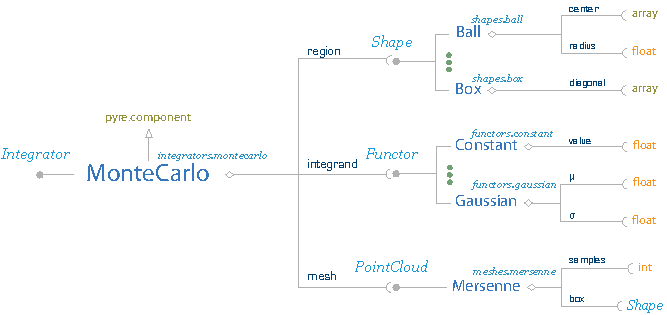
\includegraphics[scale=1.0]{figures/montecarlo.pdf}
  \end{figure}
%
\end{frame}

%-----------------------------------

\subsection{implementation}

%-----------------------------------
\begin{frame}
%
  \frametitle{Implementation strategy}
%
  \begin{itemize}
%
  \item key abstractions:
    \begin{description}
    \item[functor:] encapsulation of a function in a class; our integrands will be functors
    \item[shape:] a spatial domain; we will use these to specify the region of integration
    \item[mesh:] a discretization of the domain of integration; meshes provide the locations at
      which we sample integrands
    \item[integrator:] the implementation of a particular integration algorithm
    \end{description}
%
  \item each one of these will turn into a {\em protocol}
    \begin{itemize}
    \item that spells out all the obligations imposed on concrete realizations
    \end{itemize}
%
  \item {\em components}
    \begin{itemize}
    \item must provide concrete implementations of all the obligations
    \item specify their public state: what can be delegated to the end user
    \end{itemize}
%
  \end{itemize}
%
\end{frame}

%-----------------------------------
\begin{frame}
%
  \frametitle{Package layout}
%
  \begin{itemize}
%
  \item use the names of the abstractions to determine the directory layout
%
    \begin{columns}[t]
%
      \begin{column}{0.5\textwidth}
        \begin{figure}
          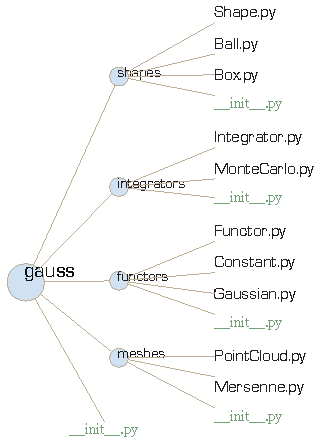
\includegraphics[scale=0.70]{figures/layout-files.pdf}
        \end{figure}
      \end{column}
%
      \begin{column}{0.5\textwidth}
        \begin{figure}
          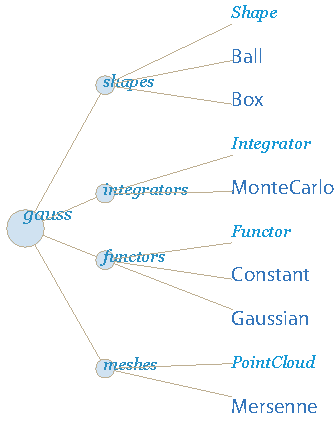
\includegraphics[scale=0.70]{figures/layout-namespace.pdf}
        \end{figure}
      \end{column}
%
    \end{columns}
%
  \item which affects the default {\em namespace} layout
%
  \end{itemize}
%
\end{frame}

%-----------------------------------
\begin{frame}
%
  \frametitle{The {\tt Shape} protocol}
%
  \vskip -1em
  \begin{itemize}
  \item in {\tt gauss/shapes/Shape.py}
    \python{firstnumber=9, linerange={9-31}}{listings/shape.py}
  \end{itemize}
%
\end{frame}

%-----------------------------------
\begin{frame}
%
  \frametitle{The {\tt Integrator} protocol}
%
  \vskip -1em
  \begin{itemize}
  \item in {\tt gauss/integrators/Integrator.py}
    \python{firstnumber=9, linerange={9-29}}{listings/integrator.py}
  \end{itemize}
%
\end{frame}

%-----------------------------------
\begin{frame}
%
  \frametitle{The {\tt MonteCarlo} integrator}
%
  \vskip -1em
  \begin{itemize}
  \item in {\tt gauss/integrators/MonteCarlo.py}
    \python{firstnumber=19, linerange={19-45}, basicstyle=\tt\tiny}{listings/montecarlo.py}
  \end{itemize}
%
\end{frame}

%-----------------------------------

\subsection{configuration}

%-----------------------------------
\begin{frame}
%
  \frametitle{User configuration}
%
  \cfg{firstnumber=7, linerange={7-23}, xleftmargin=4em}{listings/gauss.cfg}
%
\end{frame}

% end of file

% -*- LaTeX -*-
% -*- coding: utf-8 -*-
%
% michael a.g. aïvázis
% california institute of technology
% (c) 1998-2012 all rights reserved
%

%-----------------------------------

\section{applications}

% --------------------------------------
% the application harness
\begin{frame}[fragile]
%
  \frametitle{Creating an application}
%
  \vskip -3ex
  \begin{itemize}
%
  \item applications are the top level component managers
%
    \python{firstnumber=10,linerange={10-34}}{listings/quad.py}
%
  \end{itemize}
%
\end{frame}

% --------------------------------------
% the application harness
\begin{frame}[fragile]
%
  \frametitle{Auto-launching}
%
  \begin{itemize}
%
  \item instantiating and launching the application
%
    \python{firstnumber=54,linerange={54-60}}{listings/quad.py}
%
  \item a sample configuration file
%
    \cfg{firstnumber=8, linerange={8-20}}{listings/quad.cfg}
%
  \end{itemize}
%
\end{frame}

% --------------------------------------
% the application component
\begin{frame}[fragile]
%
  \frametitle{The application component}
%
  \begin{itemize}
%
  \item the shell hierarchy in pyre
%
  \begin{figure}
    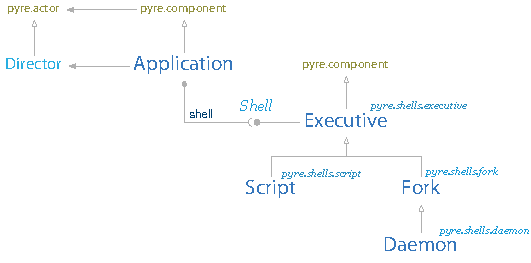
\includegraphics[scale=1.0]{figures/shells.pdf}
  \end{figure}
%
  \item our \identifier{Quad} derives from \identifier{Application}, so it has a
    \identifier{shell}
%
  \end{itemize}
%
\end{frame}

% --------------------------------------
% the parallel version
\begin{frame}[fragile]
%
  \frametitle{Parallel integration}
%
  \begin{itemize}
%
  \item the \identifier{mpi} entry point
%
    \python{firstnumber=36,linerange={36-52}}{listings/quad.py}
%
  \item the \package{mpi} package is part of the pyre distribution
    \begin{itemize}
    \item handles initialization and finalization of \package{MPI}
    \item simplifies most of the ``overhead'' activities
    \item provides an OO veneer
    \end{itemize}
%
  \end{itemize}
%
\end{frame}

% --------------------------------------
% running the mpi program
\begin{frame}[fragile]
%
  \frametitle{Running in parallel}
%
  \begin{itemize}
%
  \item minor modifications to the configuration file...
%
    \cfg{firstnumber=8, linerange={8-28}}{listings/quad.cfg}
%
  \end{itemize}
%
\end{frame}

%-----------------------------------
% end of file


% references
\begin{frame}[allowframebreak]{references}
  \frametitle{References}
  \bibliographystyle{unsrtnat}
  {\small \bibliography{references}}
\end{frame}

\end{document}

% end of file 
